\documentclass[a4paper, 14pt]{extarticle}

\usepackage[T2A]{fontenc}
\usepackage{natbib}
\usepackage{graphicx}
\usepackage[english, russian]{babel}
\usepackage{fontspec}
\usepackage{amsmath}
\usepackage{amsfonts}
\usepackage{amssymb}
\usepackage{amsthm}
\usepackage{mathtools}
\usepackage{mathrsfs}
\usepackage{icomma}
\usepackage{fullpage}
\usepackage{ulem}
\usepackage{setspace}
\usepackage{listings}
\usepackage{indentfirst}
\usepackage[left=2cm,right=1.5cm,top=2cm,bottom=2cm]{geometry}
\usepackage{xcolor}
\usepackage{float}
\usepackage{csquotes}
\usepackage{hyperref}
\usepackage{graphics}



\definecolor{urlcolor}{HTML}{0000FF} % цвет гиперссылок
\definecolor{linkcolor}{HTML}{000000} % цвет гиперссылок
\hypersetup{pdfstartview=FitH, linkcolor=linkcolor, urlcolor=urlcolor, colorlinks=true}


\setmainfont{Times New Roman}
\setlength{\parindent}{5ex}
\setlength{\parskip}{1em}
\renewcommand{\baselinestretch}{1}

\graphicspath{{images/}}


\definecolor{buzzlightyear}{HTML}{8757A5}
\definecolor{grass}{HTML}{738D06}
\definecolor{literal}{HTML}{F18A2B}
\definecolor{commentcolor}{HTML}{8E908B}

\lstdefinestyle{habrstyle}{
    backgroundcolor=\color{white},
    commentstyle=\color{commentcolor},
    keywordstyle=\bfseries\color{buzzlightyear},
    numberstyle=\tiny\color{commentcolor},
    stringstyle=\color{grass},
    basicstyle=\ttfamily\footnotesize,
    breakatwhitespace=false,
    breaklines=true,
    captionpos=b,
    keepspaces=true,
    numbers=left,
    numbersep=5pt,
    showspaces=false,
    showstringspaces=false,
    showtabs=false,
    tabsize=4
}

\lstset{style=habrstyle}

\begin{document}
    % НАЧАЛО ТИТУЛЬНОГО ЛИСТА
    \begin{center}
        \begin{center}
            \hfill \break
            \normalsize{Санкт-Петербургский государственный политехнический}\\
            \normalsize{университет Петра Великого}\\
            \hfill \break
            \normalsize{\textbf{Высшая школа интеллектуальных систем и}}\\
            \normalsize{\textbf{суперкомпьютерных технологий}}\\
            \hfill \break
            \hfill \break
            \hfill \break
            \normalsize{Лабораторная работа}\\
            \hfill \break
            \normalsize{\LARGE Автокорреляция}\\
        \end{center}
        \hfill \break
        \hfill \break
        \hfill \break
        \hfill \break
        \hfill \break
        \hfill \break
        \hfill \break
        \hfill \break
        \hfill \break
        \hfill \break
        \begin{tabbing}
            Выполнил студент гр. 3530901/80201 \`И.С. Иванов\\
            \\
            Преподаватель: \`Н.В. Богач\\
        \end{tabbing}
        \hfill \break
        \hfill \break
        \hfill \break
        \hfill \break
        \begin{center}
            Санкт-Петербург\\
            2021
        \end{center}
        \thispagestyle{empty}
    \end{center}
    % КОНЕЦ ТИТУЛЬНОГО ЛИСТА

    % ОГЛАВЛЕНИЕ
    \newpage
    \tableofcontents

    % СПИСОК ИЛЛЮСТРАЦИЙ
    \newpage
    \listoffigures

    % СПИСОК ЛИСТИНГОВ
    \newpage
    \lstlistoflistings

    \newpage


    \section{Упражнение №1}
    \label{sec:1}

    Во первом упражнении необходимо вычислить автокорреляцию для различных \texttt{lag} и оценить высоту тонна локального \texttt{chirp}.

    Создадим функции \texttt{autocorr} и \texttt{serial\_corr}

    \begin{lstlisting}[language=Python, caption=Функция serial\_corr, label={lst:serial_corr}]
        def serial_corr(wave, lag=1):
            n = len(wave)
            y1 = wave.ys[lag:]
            y2 = wave.ys[:n - lag]
            corr_mat = np.corrcoef(y1, y2)
            return corr_mat[0, 1]
    \end{lstlisting}

    \begin{lstlisting}[language=Python, caption=Функция autocorr, label={lst:autocorr}]
        def autocorr(wave):
            lags = np.arange(len(wave.ys) // 2)
            corrs = [serial_corr(wave, lag) for lag in lags]
            return lags, corrs
    \end{lstlisting}

    Прочитаем файл.
    Построим график автокорреляции.

    \begin{lstlisting}[language=Python, caption={Чтение файла, построение графика автокорреляции}, label={lst:read_plot_autocorr}]
        wave = read_wave('Sounds/28042__bcjordan__voicedownbew.wav')
        wave.normalize()
        wave.make_audio()

        segment = wave.segment(0, 0.01)
        lags, corrs = autocorr(segment)
        low, high = 90, 110
        lag = np.array(corrs[low:high]).argmax() + low
        plt.plot(lags, corrs, color='blue')
        decorate(xlabel='Lag', ylabel='Correlation')
    \end{lstlisting}

    \begin{figure}[H]
        \centering
        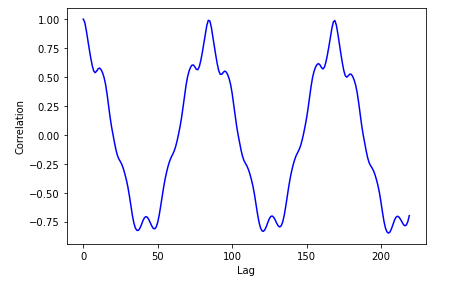
\includegraphics[width=0.8\linewidth]{autocorr_wave}
        \caption{График автокорреляции}
        \label{fig:autocorr_wave}
    \end{figure}

    На графике видно, что он периодический.
    Период равен 90.

    \newpage


    \section{Упражнение №2}
    \label{sec:2}

    Во втором упражнении необходимо написать функцию \texttt{estimate\_fundamental}, отслеживающую высоту тона записанного звука.
    Также необходимо проверить ее работоспособность.

    Напишем функцию:

    \begin{lstlisting}[language=Python, caption= Функция estimate\_fundamental, label={lst:estimate_fundamental}]
        def estimate_fundamental(segment, low=70, high=150):
            lags, corrs = autocorr(segment)
            lag = np.array(corrs[low:high]).argmax() + low
            period = lag / segment.framerate
            frequency = 1 / period
            return frequency
    \end{lstlisting}

    Посмотрим на спектрограмму аудио файла из предыдущего упражнения.

    \begin{figure}[H]
        \centering
        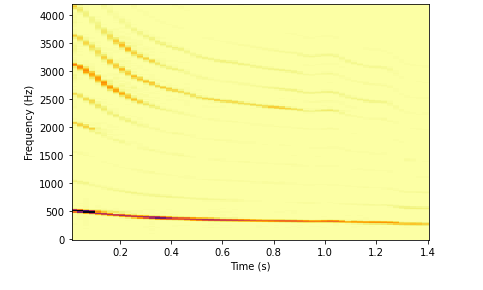
\includegraphics[width=0.8\linewidth]{wave_spectrogram}
        \caption{Спектрограмма аудио файла}
        \label{fig:wave_spectrogram}
    \end{figure}

    С помощью написанной ранее функции получим минимальную частоту сегмента.

    \begin{lstlisting}[language=Python, caption= Получение минимальной частоты сегмента, label={lst:use_estimate_fundamental}]
        duration = 0.01
        segment = wave.segment(start=0.2, duration=duration)
        freq = estimate_fundamental(segment)
        freq
    \end{lstlisting}

    Минимальная частота равна 436.63366336633663.

    Найдем этот сегмент с шагом 0.05.

    \begin{lstlisting}[language=Python, caption= Поиск сегмента с минимальной частотой, label={lst:find_segment}]
        step = 0.05
        starts = np.arange(0.0, 1.4, step)

        ts = []
        freqs = []

        for start in starts:
            ts.append(start + step/2)
            segment = wave.segment(start=start, duration=duration)
            freq = estimate_fundamental(segment)
            freqs.append(freq)
    \end{lstlisting}

    Выведем спектрограмму найденного сегмента.

    \begin{lstlisting}[language=Python, caption= Спектрограмма сегмента, label={lst:spectrogram_segment}]
        wave.make_spectrogram(2048).plot(high=900)
        plt.plot(ts, freqs, color='white')
        decorate(xlabel='Time (s)',
                             ylabel='Frequency (Hz)')
    \end{lstlisting}

    \begin{figure}[H]
        \centering
        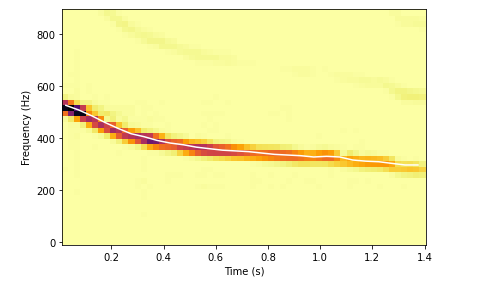
\includegraphics[width=0.8\linewidth]{segment_spectrogram}
        \caption{Спектрограмма сегмента}
        \label{fig:segment_spectrogram}
    \end{figure}

    На полученной спектрограмме можно увидеть искомую частоту.

    \newpage


    \section{Упражнение №3}
    \label{sec:3}

    В третьем упражнении нам необходимо используя данные курса Bitcoin из предыдущей лабораторной работы вычислить автокорреляцию курса.

    Считаем файл и выведем график:

    \begin{lstlisting}[language=Python, caption= Считывание файла, label={lst:read_bitcoin}]
        import pandas as pd

        df = pd.read_csv('Res/BTC_USD_2013-10-01_2021-05-04-CoinDesk.csv',
                         parse_dates=[0])

        ys = df['Closing Price (USD)']
        ts = df.index

        from thinkdsp import Wave

        wave = Wave(ys, ts, framerate=1)
        wave.plot()
        decorate(xlabel='Time (days)',
                 ylabel='Price of BitCoin ($)')
    \end{lstlisting}

    \begin{figure}[H]
        \centering
        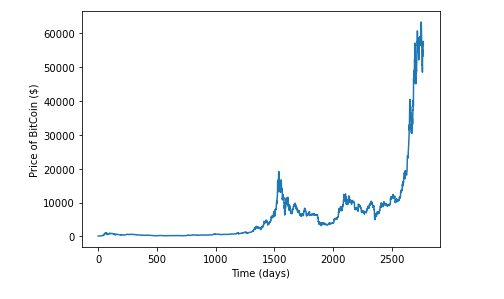
\includegraphics[width=0.8\linewidth]{bitcoin_wave}
        \caption{График курса Bitcoin}
        \label{fig:bitcoin_wave}
    \end{figure}

    Посмотрим на график функции автокорреляции.

    \begin{figure}[H]
        \centering
        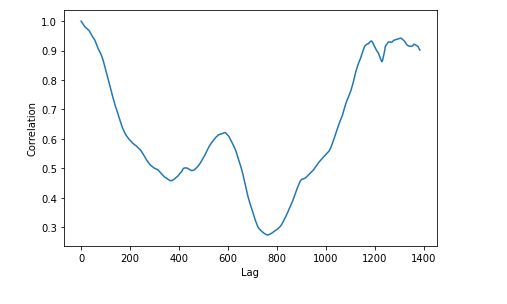
\includegraphics[width=0.8\linewidth]{bitcoin_autocorr}
        \caption{Автокорреляционный график курса Bitcoin}
        \label{fig:bitcoin_autocorr}
    \end{figure}

    Периодичности на графике не наблюдается.

    \newpage


    \section{Упражнение №4}
    \label{sec:4}

    В четвертом упражнении необходимо просмотреть файл \texttt{saxophone.ipynb}, пройтись по всем примерам, затем выбрать сегмент записи и поработать с ним.

    Построим спектрограмму данного в задании файла

    \begin{figure}[H]
        \centering
        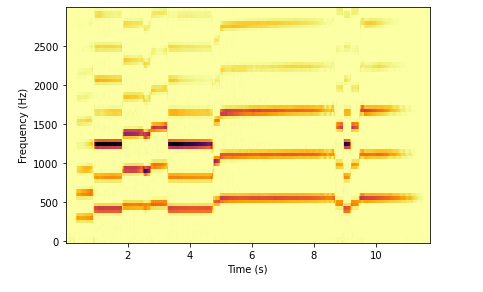
\includegraphics[width=0.8\linewidth]{sax_spectrogram}
        \caption{Спектрограмма звука саксофона}
        \label{fig:sax_spectrogram}
    \end{figure}

    Выделим сегмент отличный от исходного.
    Сегмент с 8 секунды длительностью 0.5 секунд.

    Посмотрим на спектр данного сегмента.

    \begin{figure}[H]
        \centering
        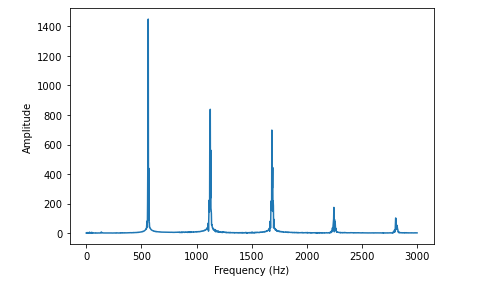
\includegraphics[width=0.8\linewidth]{sax_segment}
        \caption{Спектр сегмента саксофона}
        \label{fig:sax_segment}
    \end{figure}

    Получим "Peaks" сегмента.

    \begin{lstlisting}[language=Python, caption= Peaks, label={lst:peaks}]
        [(1449.7324059418409, 562.0),
         (838.6796549940561, 1124.0),
         (760.4866790380277, 1120.0),
         (697.9180739586471, 1682.0),
         (562.4385733324308, 1128.0),
         (548.2317169052268, 1684.0),
         (490.9435713084754, 1122.0),
         (479.5263999004895, 558.0),
         (444.5487141915133, 1690.0),
         (439.8651374537576, 566.0)]
    \end{lstlisting}

    Построим треугольный сигнал основной частоты.

    \begin{lstlisting}[language=Python, caption= Создание треугольного сигнала, label={lst:create_triangle_signal}]
        from thinkdsp import TriangleSignal

        TriangleSignal(freq=562).make_wave(duration=0.5).make_audio()
    \end{lstlisting}

    Обновим функцию автокорреляции

    \begin{lstlisting}[language=Python, caption= Обновление функции autocorr, label={lst:update_autocorr}]
        def autocorr(segment):
            corrs = np.correlate(segment.ys, segment.ys, mode='same')
            N = len(corrs)
            lengths = range(N, N//2, -1)

            half = corrs[N//2:].copy()
            half /= lengths
            half /= half[0]
            return half
    \end{lstlisting}

    Выведем на экран график автокорреляции звукового сегмента.

    \begin{lstlisting}[language=Python, caption= Вывод графика автокорреляции, label={lst:sax_autocorr}]
        corrs = autocorr(segment)
        plt.plot(corrs[:200])
        decorate(xlabel='Lag', ylabel='Correlation', ylim=[-1.05, 1.05])
    \end{lstlisting}

    \begin{figure}[H]
        \centering
        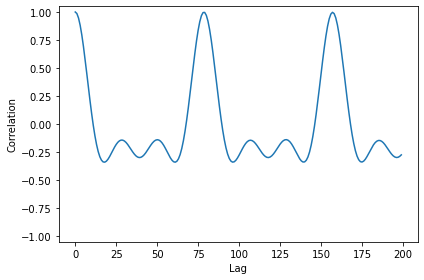
\includegraphics[width=0.8\linewidth]{sax_autocorr}
        \caption{График автокорреляции сегмента звука саксофона}
        \label{fig:sax_autocorr}
    \end{figure}

    На графике видно, что первый наибольший пик на значении 80.
    Для нахождения частоты напишем функцию.

    \begin{lstlisting}[language=Python, caption= Функция find\_frequency, label={lst:find_frequency}]
        def find_frequency(corrs, low, high):
            lag = np.array(corrs[low:high]).argmax() + low
            print(lag)
            period = lag / segment.framerate
            frequency = 1 / period
            return frequency
    \end{lstlisting}

    \begin{lstlisting}[language=Python, caption= Вызов find\_frquency, label={lst:call_find_frequency}]
        find_frequency(corrs, 70, 95)
    \end{lstlisting}

    Самый большой \texttt{lag} = 79.
    Частота 558.2278481012657.

    Необходимо отфильтровать сегмент с помощью фильтра низких частот.

    \begin{lstlisting}[language=Python, caption= Фильтрация сегмента, label={lst:high_pass}]
        spectrum2 = segment.make_spectrum()
        spectrum2.high_pass(600)
        spectrum2.plot(high=3000)
        decorate(xlabel='Frequency (Hz)', ylabel='Amplitude')
    \end{lstlisting}

    \begin{figure}[H]
        \centering
        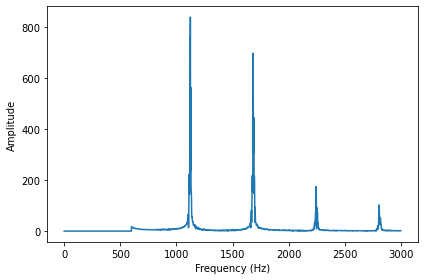
\includegraphics[width=0.8\linewidth]{sax_filtered_spectrum}
        \caption{Спектр отфильтрованного сегмента саксофона}
        \label{fig:sax_filtered_spectrum}
    \end{figure}

    На спектре можно увидеть, что основная частота была убрана.

    Сравнив звук исходного фрагмента и отфильтрованного можно сказать, что отфильтрованный звучит приглушеннее, так как убраны низкие частоты.

    \newpage


    \section{Выводы}
    \label{sec:conclusions}

    В результате выполнения данной лабораторной работы мы изучили, понятие автокорреляции.
    Была создана функция \texttt{estimate\_fundamental} для отслеживания высоты тона звука.
    Была вычислена автокорреляция курса валют \texttt{Bitcoin} из прошлой лабораторной работы.
    Была произведена работа по вычислению значения автокорреляции для сегмента записи саксофона.

\end{document}